% document formatting
\documentclass[10pt]{article}
\usepackage[utf8]{inputenc}
\usepackage[left=1in,right=1in,top=1in,bottom=1in]{geometry}
\usepackage[T1]{fontenc}
\usepackage{xcolor}

% math symbols, etc.
\usepackage{amsmath, amsfonts, amssymb, amsthm}
\usepackage{mathtools}

% lists
\usepackage{enumerate}

% images
\usepackage{graphicx} % for images
\usepackage{multirow}

% code blocks
\usepackage{minted, listings} 

% verbatim greek
\usepackage{alphabeta}

\graphicspath{{./assets/images}}

\newcommand{\solution}{\textbf{Solution:}} 
\newcommand{\example}{\textbf{Example: }}
\newcommand{\sinc}{\text{sinc}}
\newcommand{\rect}{\text{rect}}
\newcommand{\llra}{\Longleftrightarrow}
\newcommand{\fourier}{\mathcal{F}}
\newcommand{\absint}{\int_{-\infty}^\infty}
\newcommand{\dd}{\text{d}}

\title{EC ENGR 102 Week 8}

\author{Aidan Jan}
\date{\today}

\begin{document}
\maketitle

\section*{Distortions}
\subsection*{Causal Filters}
Ideal filters are not causal.
\begin{itemize}
    \item The impulse responses of the ideal low pass, high pass, and band pass filters are all non-causal.  This is obviously not practical in real-time scenarios, where the future is not known.
    \item To this end, it seems we have a problem.  If we can't implement non-causal filters, then there has to be some approximations made (beyond introducing transition bands).
    \item What we ought to recognize is that we will never be able to take a signal at time $t$, given by $x(t)$, and immediately filter it.  However, we could wait a bit of time, and then filter $x(t)$.  This enables us to implement a causal filter, with the con being that the signal is delayed.
\end{itemize}
A practically implementable system that is causal must introduce a delay.  For example, we could implement a practical and causal low pass filter by taking the impulse response of the ideal low pass filter, and:
\begin{itemize}
    \item Truncate it (so that it is zero for some time $|t| > t_d$).
    \item Delay it by time $t_d$ so that it is causal.
\end{itemize}
This is illustrated below:
\begin{center}
    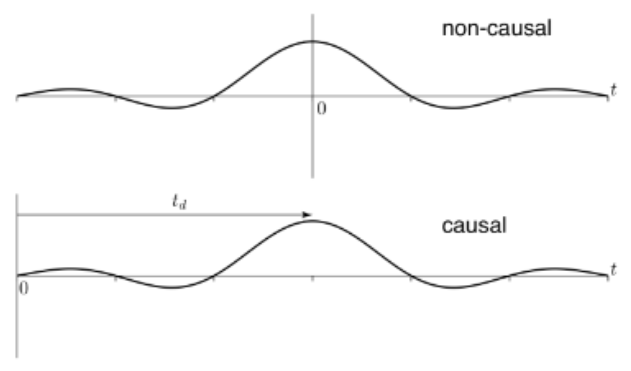
\includegraphics[width=\textwidth]{W8_1.png}
\end{center}
\subsection*{Distortionless LTI Systems}
When using filters, distortion could be introduced.  In the frequency domain, depending on the filter being used, components of the signal at different frequencies may be amplified differently or may be delayed.  We know that filtering causes:
\begin{itemize}
    \item Amplitude scaling by $|H(j\omega)|$
    \item Phase shifting by $\angle H(j\omega)$
\end{itemize}
and depending on the frequencies of the signal, this could cause distortion to the system.\\\\
A system is without distortion if
\[y(t) = Kx(t - t_d)\]
where $K$ is a scaling factor and $t_d$ is a delay.  This tells us that a distortionless signal is one that is identical to the input signal up to amplification and a constant delay.\\\\
What is $H(j\omega)$ for a distortionless LTI system?\\\\
This is a system with 
\[|H(j\omega)| = K\]
and
\[\angle H(j\omega) = -\omega t_d\]
It has the following amplitude and phase spectra:
\begin{center}
    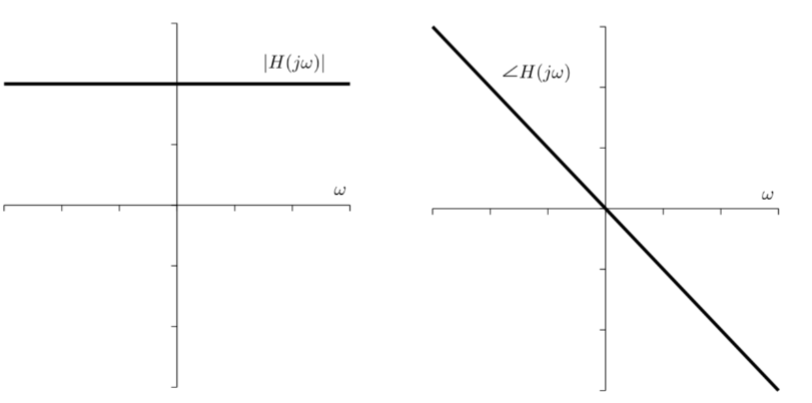
\includegraphics[scale=0.5]{W8_2.png}
\end{center}
\subsection*{Amplitude Distortion}
Amplitude distortion is relatively straightforward.
\begin{center}
    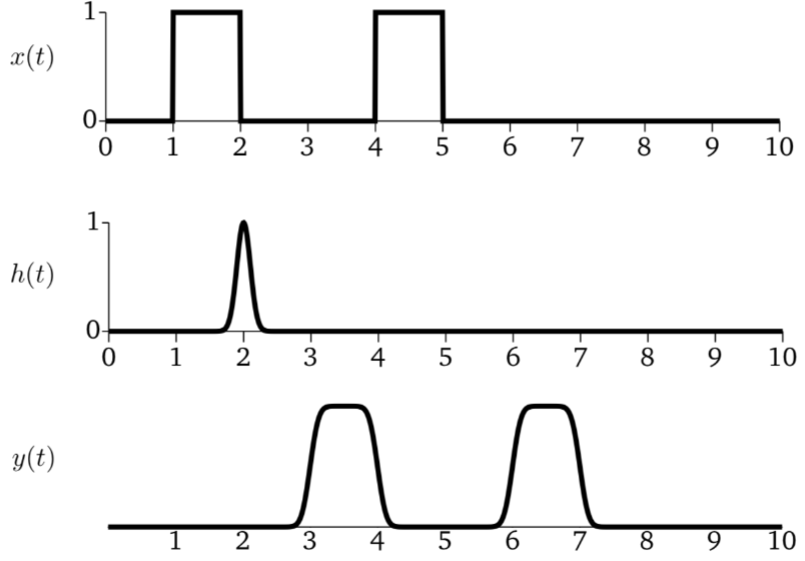
\includegraphics[scale=0.5]{W8_3.png}
\end{center}
If we have an impulse which is not really an impulse (due to real life physics limitations), we get some distortion in the output.
\subsection*{Phase Distortion}
\begin{center}
    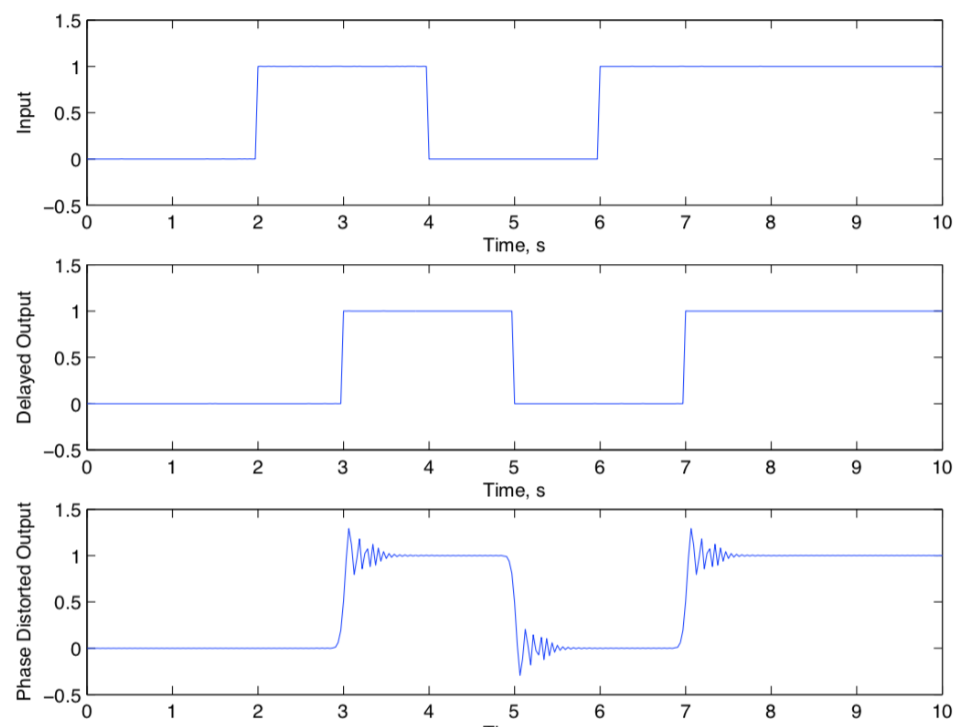
\includegraphics[scale=0.8]{W8_4.png}
\end{center}
\begin{itemize}
    \item Phase distortion is caused when the different complex exponentials that compose a function are changed by slightly different frequencies, so when they sum together, something weird happens.
    \item Think: Suppose $\angle(Y(j\omega)) = \angle(x(j\omega)) + \angle(h(j\omega))$.  If a distortion in phase is made to both $x$ and $h$, does $Y$ move by the same amount?  Especially with a frequency change, they may not line up well. 
\end{itemize}
\subsection*{Group Delay}
We know that convolution with $\delta(t - t_d)$ only delays the signal, but introduces no distortion.  Further, $\fourier[\delta(t - t_d)] = e^{-j\omega t_d}$, and so its phase is
\[\angle H(j\omega) = -\omega t_d\]
It turns out that if the phase is linear, the signal is only delayed in time without distortion.\\\\
Consider a simple example, a signal $x(t) = \cos(\omega t) + \cos(2\omega t)$.  Delaying this signal by $\pi / \omega$, i.e., $y(t) = x(t) * \delta(t - \pi - \omega)$ gives
\begin{align*}
    y(t) &= \cos(\omega(t - \pi/\omega)) + \cos(2\omega(t - \pi / \omega))\\
    &= \cos(\omega t - \pi) + \cos(2\omega t - 2\pi)
\end{align*}
This makes intuitive sense, if the signal is higher frequency, we need a larger phase shift to gain the same temporal offset.\\\\
When the phase is not linear, different frequencies will experience different temporal delays.  Therefore, the amount of delay will be frequency dependent, i.e., $t_d$ will be a function of $\omega$.  Since $\angle H(j\omega) = -\omega t_d$, it is straightforward to derive what the frequency-dependent temporal delay is, i.e., it's
\[t_d(\omega) = -\frac{\dd}{\dd \omega} \angle H(j\omega)\]
From this, we can see that if $\angle H(j\omega)$ is a line with slope $-k$, then its derivative is simply $-k$, leading to every frequency having the same delay $t_d = k$.  This confirms our intuition from before.\\\\
This quantity, $t_d(\omega)$, is called \textit{group delay}.
\subsection*{Distortions}
Importance of amplitude and phase distortion depends on application.\\\\
For audio or speech:
\begin{itemize}
    \item Amplitude distortion is very is important.
    \item Humans are relatively insensitive to phase distortion.
\end{itemize}
For images or video:
\begin{itemize}
    \item Amplitude distortion is relatively unimportant, as long as it is slowly varying.
    \item Phase distortion is very important.  Small amounts of non-linear phase result in very blurry looking images.
\end{itemize}
\section*{Sampling}
\subsection*{Motivation}
In reality, we could never store a continuous time signal.  Instead, as we see in \texttt{MATLAB}, we store a signal's value at various times.\\\\
A key variable of interest is the sampling frequency, i.e., the time in between our samples, denoted $T$ in the above diagram.\\\\
This is related to discrete signals, i.e., $x[n] = x(nT)$.
\subsection*{How to sample a continuous signal?}
How do we sample a continuous signal?  You may have several intuitions to do so already using the $\delta(t)$ signal and its property that $f(t) \delta(t) = f(0) \delta(t)$.
\begin{itemize}
    \item We will arrive at sampling by first studying a related problem: the Fourier transform of periodic signals.
    \item The reason we approach this is that Fourier series are discrete coefficients, $c_k$, while the Fourier transform is typically some continuous signal.  i.e., it seems like there may be a relationship whereby the Fourier series is like a sampled Fourier transform.
    \item So we ask: what is the relationship between the Fourier series and the Fourier transform?
    \item To see this, we can begin by identifying the relationship between the Fourier series and the Fourier transform.
\end{itemize}
\subsection*{Fourier transform of a periodic signal}
We cannot directly take the Fourier transform of a periodic signal, since they do not have finite energy.  However, we can use a few tricks (like in the Generalized Fourier Transform lecture) to calculate the FT of a periodic signal.\\\\
Let $f(t)$ have a Fourier series (with period $T_0 = \omega_0/2\pi$)
\[f(t) = \sum_{k = -\infty}^\infty c_k e^{jk\omega_0 t}\]
with 
\[c_k = \frac{1}{T_0} \int_{0}^{T_0} f(t) e^{jk\omega_0 t} \dd t\]
There's a close relationship between the two, as the Fourier series equation looks like the Fourier transform equation but with a $\sum$ instead of an $\int$.
\begin{center}
    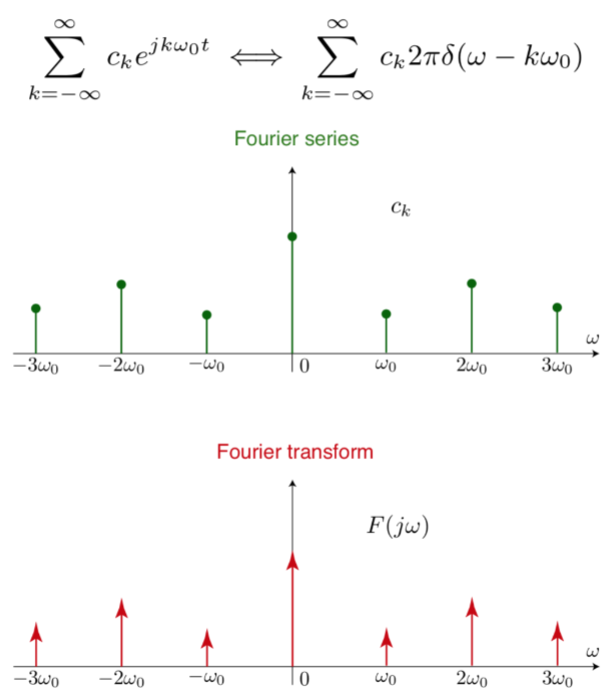
\includegraphics[scale=0.6]{W8_5.png}
\end{center}
\example\\
Consider the square wave below:
\[f(t) = \sum_{k=-\infty}^\infty \rect(t - 2k)\]
This is illustrated below:
\begin{center}
    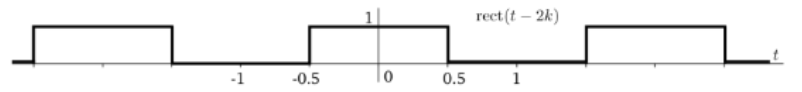
\includegraphics[width=\textwidth]{W8_6.png}
\end{center}
In the Fourier series lecture (slides 8-32), we calculated that the Fourier series of this signal is:
\[c_k = \frac{1}{2}\sinc(k/2)\]
What is its Fourier transform?
\[\sum_{k=-\infty}^\infty c_k e^{jk\omega_0 t} \llra \sum_{k=-\infty}^\infty c_k 2\pi \delta(\omega - k\omega_0)\]
\[F(j\omega) = \sum_{k=-\infty}^\infty \frac{1}{2} \sinc\left(\frac{k}{2}\right) \cdot 2\pi \cdot \delta(\omega - k\pi)\]
The $\delta(\omega - k\pi)$ is an impulse at $\omega = k\pi$.  Therefore, $k = \frac{\omega}{\pi}$.\\\\
Hence, the Fourier transform of the square wave is the Fourier transform of a $\rect$ multiplied by evenly spaced $\delta$'s, i.e.,
\begin{align*}
    F(j\omega) &= \pi \sum_{k=-\infty}^\infty \sinc(\omega/2\pi) \delta(\omega - k\pi)\\
    &= \pi \cdot \sinc(\omega/2\pi) \cdot \sum_{k=-\infty}^\infty \delta(\omega - k\pi)\\
\intertext{Impulse train notation: (this is discussed below.)}
    &= \pi \cdot \sinc\left(\frac{\omega}{2\pi}\right) \cdot \delta_\pi(\omega)
\end{align*}
\begin{center}
    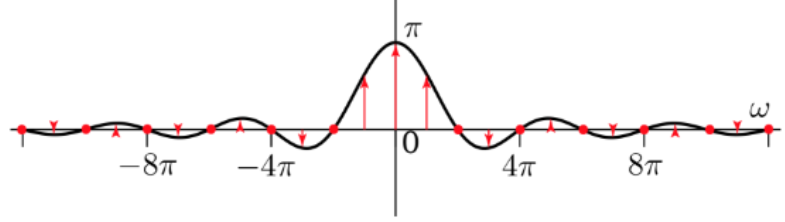
\includegraphics[width=\textwidth]{W8_7.png}
\end{center}
\subsubsection*{Impulse Trains}
To simplify the notation here, we can define an \textit{impulse train} which ends up being our sampling function.  We let $\delta_T(t)$ be a sequence of unit $\delta$ functions spaced by $T$.
\[\delta_T(t) = \sum_{k=-\infty}^\infty \delta(t - kT)\]
This is illustrated below:
\begin{center}
    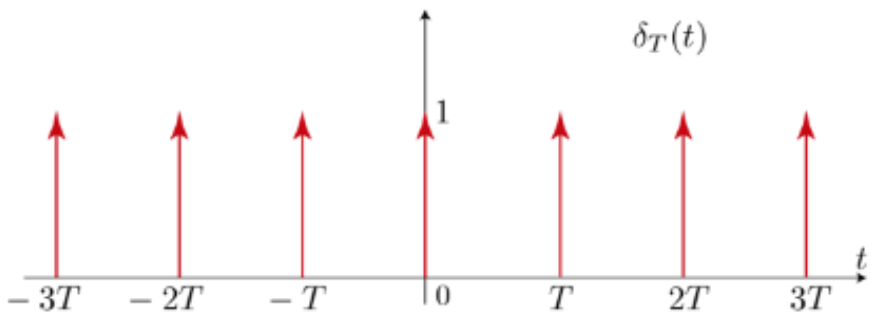
\includegraphics[width=\textwidth]{W8_8.png}
\end{center}
\subsection*{Fourier Series of Impulse Train}
By intuition:
\begin{itemize}
    \item We know that the Fourier transform of the square wave is a $\sinc$ multiplied by a $\delta_\pi(\omega)$.
    \item From the convolution theorem, this means that the inverse Fourier transform (i.e., the square wave) is the inverse Fourier transform of a $\sinc$ convolved with the inverse Fourier transform of a impulse train.
    \item We know that a square is simply a $\rect$ repeated over and over again, i.e., convoluted with a impulse train.
    \item So intuitively, the Fourier transform of a impulse train should be a impulse train.
    \item Note: we will sometimes use the term 'delta train' to describe an impulse train.
\end{itemize}
Proof:
\begin{align*}
    c_k &= \frac{1}{T} \int_{\text{1 period}} f(t) e^{-jk\omega_0 t} \dd t\\
    &= \frac{1}{T} \int_{-\frac{T}{2}}^{\frac{T}{2}} \delta_T(t) \cdot e^{-jk\omega_0 t} \dd t\\
    \intertext{Note that $\omega_0 = 2\pi/T$}
    &= \frac{1}{T} \int_{-\frac{T}{2}}^{\frac{T}{2}} \delta(t) e^0 \dd t\\
    \Aboxed{c_k &= \frac{1}{T}}
\end{align*}
Therefore,
\begin{align*}
    \fourier[\delta_T(t)] &= \fourier\left[\frac{1}{T} \sum_{k=-\infty}^\infty e^{jk\omega_0 t}\right]\\
    &= \frac{1}{T} \sum_{k=-\infty}^\infty \fourier\left[e^{-jk\omega_0 t}\right]\\
    \intertext{Recall that $e^{jk\omega_0 t} \llra 2\pi \cdot \delta(\omega - k\omega_0)$.}
    &= \frac{1}{T} \sum_{k=-\infty}^\infty 2\pi \cdot \delta(\omega - k\omega_0)\\
    &= \omega_0 \cdot \delta_{\omega_0}(\omega)
\end{align*}
By this, the Fourier transform of an impulse train is an impulse train.
\subsection*{Sampling with an impulse train}
As we saw earlier, one of the things we will use the impulse train for is to sample signals.\\\\
Given a signal $f(t)$,
\begin{align*}
    f(t) \delta_T(t) &= f(t) \cdot \sum_{k=-\infty}^\infty \delta(t - kT)\\
    &= \sum_{k=-\infty}^\infty f(t) \cdot \delta(t - kT)\\
    \Aboxed{\hat{f}(t) &= \sum_{k=-\infty}^\infty f(kT) \cdot \delta(t - kT)}
\end{align*}
\subsection*{Square Wave Example pt. 2}
Let's revisit our square wave example, where
\[f(t) = \sum_{k=-\infty}^\infty \rect(t-2k)\]
Another way to represent this square wave is as follows:
\[f(t) = \rect(t) * \delta_2(t)\]
Hence, we can calculate its Fourier transform by using the convolution theorem.  Recall that, for $\omega_0 = 2\pi/T$.
\[\rect(t) \llra \sinc(\omega/2\pi)\]
and
\[\delta_T(t) \llra \omega_0 \delta_{\omega_0} (\omega)\]
Note that when $T = 2$, then $\omega_0 = \pi$.  Then, we have that,
\begin{align*}
    \fourier[f(t)] &= \fourier[\rect(t) * \delta_2(t)]\\
    &= \fourier[\rect(t)] \fourier[\delta_2(t)]\\
    &= \sinc(\omega/2\pi) \pi \delta_\pi(\omega)
\end{align*}
This is exactly the same Fourier transform we calculated earlier using the Fourier series of the square wave.
\subsection*{Sampling and Periodicity}
Another intuition to remember here is that the Fourier transform of a periodic signal is the Fourier transform of one period of the signal (which we can denote $f_1$), sampled by an impulse train at multiples of $\omega_0$.
\begin{center}
    \includegraphics*[width=\textwidth]{W8_9.png}
\end{center}
\textbf{Discrete - periodic duality}\\\\
We can determine the Fourier transform of a signal sampled in the time domain.  Consider
\[\tilde{f}(t) = f(t) \delta_T(t)\]
Its Fourier transform is
\[\tilde{F}(j\omega) = \fourier[f(t) \delta_T(t)]\]
These are merely samples of $F(j\omega)$ repeated every $\omega_0$, since
\[\tilde{F}(j\omega) = \frac{1}{T} F(j\omega) * \delta_{\omega_0}(\omega)\]

\end{document}